\documentclass[10]{edrfcm}

% EDRFCM2026 two-page extended abstract.
% Venue: Universidad Carlos III de Madrid (Puerta de Toledo), 8--11 Sept 2026.

\usepackage{graphicx}
\usepackage{amsmath}
\usepackage{amssymb}
\usepackage{stfloats}
\usepackage[numbers,sort&compress]{natbib}

\newcommand{\avg}[1]{\langle{#1}\rangle}
\newcommand{\omegaz}{\omega_z}
\renewcommand\bibsection{%
   \par\vspace{16pt}
   \noindent\textsf{\textbf{\MakeUppercase{References}}}%
   \par\vspace{2pt}}

%%%%%%%%%%%%%%%%%%%%%%%%

\title{Forecastable and Observable Reduced-Order States for Extreme Vortex-Gust Airfoil Interactions}

\author{
	\textbf{Alberto Solera-Rico}$^{1,2}$,
	\textbf{Arnau Mir\'o}$^{3,4}$,
	\textbf{Oriol Lehmkuhl}$^{4}$,
	\textbf{Carlos Sanmiguel Vila}$^{1,2*}$
	\\[6pt]
	$^{1}$Aerial Platforms Department, Spanish National Institute for Aerospace Technology (INTA), San Mart\'in de la Vega, Madrid, Spain \\
	$^{2}$Department of Aerospace Engineering, Universidad Carlos III de Madrid (UC3M), Legan\'es, Madrid, Spain \\
	$^{3}$TUAREG, Universitat Polit\`ecnica de Catalunya (UPC), Terrassa, Spain \\
	$^{4}$Barcelona Supercomputing Center (BSC), Barcelona, Spain
}

\corrauthor{$^{*}$Corresponding author: \texttt{csanvil@inta.es}}

\keywords{AI and data-driven flow control, Flow separation control, Active flow control}

%%%%%%%%%%%%%%%%%%%%%%%

\begin{document}
\maketitle

\begin{figure*}[b]
\centering
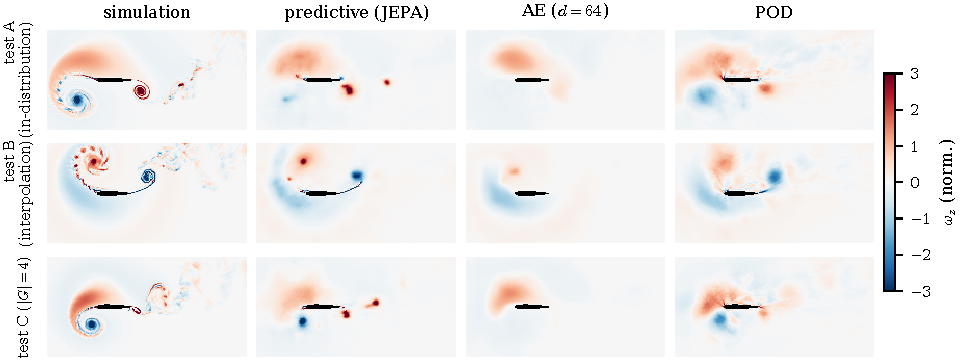
\includegraphics[width=0.86\textwidth]{Figures/decode_splits.pdf}
\caption{Decoded vorticity at the impact frame. Rows: a
test\,A (in-distribution held-out) encounter at $(G,D,Y) = (+3.0,1.5,+0.2)$, a
test\,B (interpolation) encounter at $(-3.0,1.5,-0.1)$, and a test\,C
(extrapolation, $|G| = 4$) encounter at $(+4.0,1.0,+0.1)$, each the strongest gust
in its split. Columns: the simulation, the predictive (JEPA) decode, the matched
autoencoder (AE, $d = 64$), and POD.}
\label{fig:decode}
\end{figure*}

\section{Introduction}

Extreme vortex-gust encounters generate rapid aerodynamic-load transients through
the formation and shedding of leading-edge vortices, a regime relevant to small
air vehicles where the gust velocity rivals the flight speed. The response depends
on the nonlinear interaction between the incoming vortex, the separated wake, and
the phase of the natural shedding cycle \cite{fukami2024control}.

A useful reduced-order state must do two things: retain the vortical structures
that govern the transient, and remain predictive when evolved forward, since
forecasting depends on the future state rather than its instantaneous
reconstruction. Proper orthogonal decomposition (POD) and nonlinear autoencoders
(AEs) are designed to reconstruct the field; whether their coordinates also form a
dynamically consistent state for gust evolution is less clear.

We compare three reduced-order states: a linear POD basis, an AE \cite{fukami2025},
and a joint-embedding predictive architecture (JEPA) \cite{lejepa} trained to
predict the future reduced state directly, without reconstructing the field. The
question is not which reconstructs the flow best, but which provides a compact
state whose forward evolution preserves the organisation of the gust encounter.


\section{Methodology}

The study uses direct numerical simulations at $Re = 5000$ of a NACA~0012 at
$\alpha = 14^{\circ}$ (post-stall), computed with the high-order solver SOD2D.
A transient gust is introduced as an idealised inflow perturbation emulating
localised unsteady loading: a discrete Taylor vortex of strength $G$, core
diameter $D$, and wall-normal offset $Y$ convects onto the leading edge and forms
a transient leading-edge vortex. The ensemble spans $84$ cases, about $378$
encounters: training cases, a held-out in-distribution set ($42$ encounters), and
a $|G| = 4$ extrapolation set ($24$). 

To compare methodologies, three encoders map
the mid-plane spanwise vorticity field, $\omega_z(x,y,t)$, to a latent $\mathbf{z} \in \mathbb{R}^{d}$
at two matched budgets, $d = 32$ and $d = 64$: a predictive joint-embedding
architecture (JEPA), an AE after \cite{fukami2025}, and
POD. A JEPA does not reconstruct the field; it encodes each frame through a
convolutional stem and a small vision transformer over the resulting field
patches, $\mathbf{z}_t = E_\theta(\omegaz^{t})$, and trains a predictor $P_\phi$ to
advance the latent in time, scoring the prediction in the latent space. With
conditioning $\mathbf{c} = (G,D,Y)$ the objective is
\begin{equation}
\mathcal{L} = \sum_t \big\lVert P_\phi(\mathbf{z}_{\le t}, \mathbf{c})
- \mathbf{z}_{t+1} \big\rVert^2 + \lambda_{\mathrm{R}}\, \mathcal{R}(\{\mathbf{z}_t\})
+ \lambda_{\mathrm{o}}\, \mathcal{L}_{\mathrm{obs}},
\label{eq:loss}
\end{equation}
a latent-prediction error (with a scheduled-sampling rollout term); an
anti-collapse regulariser $\mathcal{R}$ (a characteristic-function penalty matching
the latent distribution to an isotropic Gaussian, preventing collapse); and a
small auxiliary loss
$\mathcal{L}_{\mathrm{obs}}$ from two heads reading off the latent the lift $C_L$
and an $80$-dimensional wake descriptor (signed patch energies over the wake
region plus a $16$-bin radial power spectrum), after the observable-augmentation
line. No term reconstructs the field. The AE carries the lift head but not the
wake head, so the comparison is between families as configured; matched-supervision
ablations attribute the wake gain to the predictive objective with wake supervision.

A single conditional transformer predictor, of the same architecture and training
fit to each encoder's own latents, advances the latent conditioned on $\mathbf{c}$
through identity-initialised adaptive layer normalisation; a common probe reads
the observables, so that only the encoder differs. We judge each state by
\emph{forward physical closure}: rolling that predictor $H = 16$ convective steps
from impact and reading six observables off the rolled-out latent, the force
coefficients $C_L$ and $C_D$, the vertical impulse $I_y$, the wake enstrophy
($\int_{\mathrm{wake}} \omegaz^{2}\,\mathrm{d}A$) and the signed circulations
$\Gamma^{\pm}$, compared to the simulation. These combine body-force, integral and
distributed-wake information. Reconstruction quality is reported but is not the
primary metric.

\section{Results}

\begin{figure*}[t]
\centering
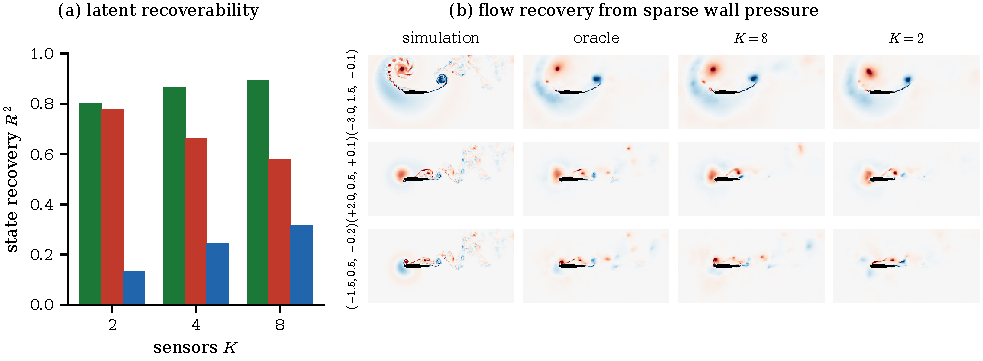
\includegraphics[width=0.77\textwidth]{Figures/observability.pdf}
\caption{Observability of the reduced state. (a) Held-out latent recovery $R^2$
from $K \in \{2,4,8\}$ TCSI wall-pressure taps at matched $d = 64$ (JEPA green,
AE red, POD blue); the predictive state is the most recoverable at
every $K$.
(b) Flow recovered on three held-out encounters (rows $(G,D,Y)$): simulation,
oracle decode (decoder on the full-field latent), and the predictive latent
estimated from $K = 8$ and $K = 2$ taps; eight taps recover the leading-edge
vortex close to the oracle, two the gross impingement.}
\label{fig:obs}
\end{figure*}

The representations differ first in what they retain. Figure~\ref{fig:decode}
shows decoded impact-frame vorticity for held-out encounters: the predictive
representation preserves the leading-edge-vortex impingement and wake organisation
more consistently than the AE, which smooths or collapses the vortical structures,
while POD is amplitude-accurate but misplaces the dominant vortices. The
$|G| = 4$ case is hardest for all three, consistent with the mid-plane
representation near a more three-dimensional regime.

The more important distinction appears under forward evolution. With the common
predictor, the predictive representation gives the most consistent closure of the
wake observables, especially wake enstrophy and signed circulation. This is not
merely better instantaneous reconstruction; it is geometric. Under rollout the AE
latent progressively leaves the region of latent space occupied by the training
data, whereas the predictive state stays near its learned manifold, and this
reduced drift preserves wake information over the horizon.

Finally, the states can be estimated online from sparse wall pressure. A
target-conditioned procedure (TCSI) selects a few surface taps and uses their
pre-impact histories to estimate the latent. The predictive state is the most
recoverable of the three (Figure~\ref{fig:obs}a); from eight taps it retains the
leading-edge vortex and shear layer close to the full-field oracle, and two taps
capture the gross impingement (Figure~\ref{fig:obs}b).

\section{Conclusions}

Reconstruction accuracy alone is not sufficient: a state that reconstructs the
instantaneous field may still fail when propagated forward if its latent geometry
is incompatible with the flow dynamics. Representations trained around future
evolution provide a more forecastable wake state, supported by several
diagnostics: reduced rollout drift, a simpler cyclic organisation of the
encounter, agreement with optimal-transport measures of vortical motion, and
better recovery from wall pressure. Forecastability and observability appear to be
closely related properties of a physically meaningful reduced-order state.


\section{Acknowledgments}

Work produced with the support of a 2024 Leonardo Grant for Researchers and
Cultural Creators, BBVA Foundation, project PREVENT grant
n.\,LEO24-2-15988-ING-ING-203. The Foundation takes no responsibility for the
opinions, statements and contents of this project, which are entirely the
responsibility of its authors.

%==================================================
\bibliographystyle{unsrtnat}
\bibliography{refs_edrfcm}

\end{document}
